%template for simulation report

\newpage

\section{Vela pulsar wind nebula}

\textbf{Object Description:} Vela pulsar and nebula

\textbf{Simulation Period:} April 2011

\textbf{NuSIM revision:} 260

\textbf{Science Team contact:} Stephen Reynolds

\textbf{NuSIM configuration file:} Vela.cfg

\textbf{Exposure time:} 200 ks

\textbf{Input Source:} 
Chandra image (cut to only include pulsar): Vela.smallerimage.fits.
Flux: $F = 6.8\cdot10^{-5}\,(E/10\,keV)^{-1.4}\,ph\,cm^{-2}\,s^{-1}\,keV^{-1}$.

\textbf{Tiling Method:} Single pointing

\textbf{OA Database Version:} 008

\textbf{Mast Bend Database:} SAA90

\textbf{Simulation notes:} While the input image has been cut down to the pulsar as good as possible, this cut is rectangular and thus not perfect. The remainig (Chandra) background around the pulsar has the same flux as the pulsar and counts towards total flux.

\textbf{Status:} 
Redo when improved depth cuts are available

\textbf{Location and name of simulation output:} resource/examples/Vela

\begin{figure}[h]
\begin{center}
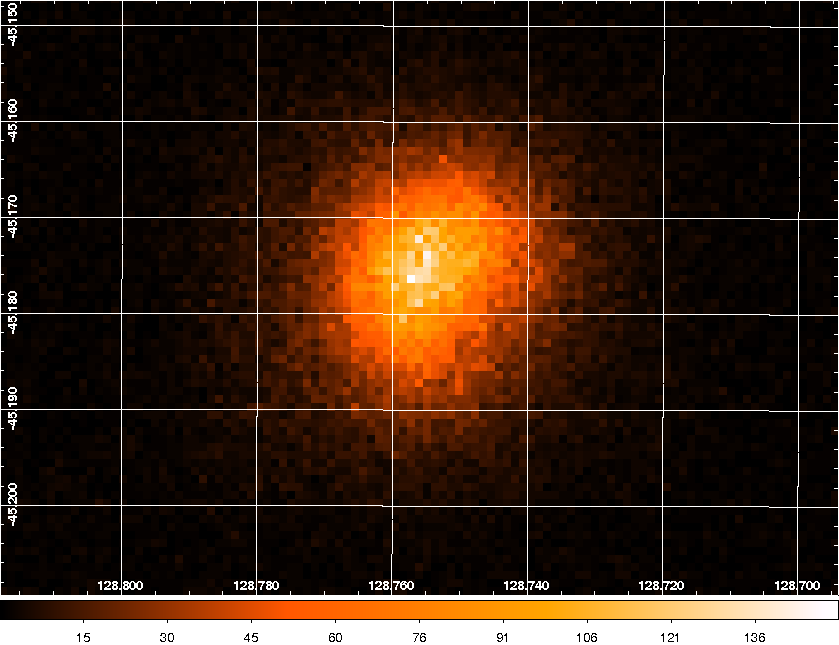
\includegraphics[width=14cm]{Vela/Vela.png}
\caption{Vela PWN between 10 and 40 keV after 200 ks observation time}
\label{Vela} 
\end{center}
\end{figure}

